\chapter{序論} \label{chapter:introduction}


%%%%%%%%%%%%%%%%%%%%%%%%%%%%%%%%%%%%%%%%%%%%%%%%%%%%%%%%%%%%%%%%%%%%%%%%%%%%%%%%
\section{背景} \label{section:backglound}

\index{うえだ@上田} %消すとコンパイルできない
人間による操縦を必要とせず、自律的に活動するロボットに対する社会の期待が高まっている。
自律ロボットの活躍が期待される場所は多岐に渡り、従来のロボットのように工場のラインだけでなく、住宅や商業施設、あるいは被災地のような極限環境も含まれる。
ロボットには様々な種類が存在するが、中でも自律移動ロボットは、病院内の搬送や空港の警備などの用途で、すでに社会実装されたものも多く存在する。

これらの環境で移動ロボットが自律的に活動するためには、自己位置や周辺環境の把握と行動計画を行う必要がある。
実世界で活動するロボットは、自身の位置を直接知ることはできない。 %あとで
したがって、搭載したセンサを用いて自身の位置や周辺環境を把握する必要がある。
そして、ロボットは把握した自己位置や環境の情報を頼りに、目標地点へと移動するための行動を計画し動作する。

しかしながら、移動ロボットの活躍が求められている環境の多くは複雑で、不確かな要素が多く存在する。
人間の生活する空間は、工業の組み立てラインのように不確かさや誤差がなるべく小さくなるように精密に構成されてはいない。
また、センサが知覚できる情報には限りがありノイズが含まれているため、ロボットが環境の情報を完全に知覚することはできない。
アクチュエータにおいても、制御ノイズや消耗のような要因から誤差が存在し、モデル化やアルゴリズムの近似による誤差も存在する。
したがって、ロボットが実世界で自律的に活動するためには、これら多くの不確かさに対処していく必要がある。

不確かさを考慮するためには、確率論に基づく方法が有効である。
ロボティクスにおいて、確率論を用いて不確かさに対処する試みは「確率ロボティクス(Probabilistic Robotics)」と呼ばれ、盛んに研究が行われている\cite{thrun2005,上田2007prob}。
確率ロボティクスは、ロボットの知覚と制御に確率・統計を駆使することで、ロボット技術において避けて通ることができない不確かさを陽に表現することを可能としている。
移動ロボットにおいて重要な自己位置推定や行動計画についても、不確かさを考慮した様々なアルゴリズムが提案されている。

この確率論に基づく自己位置推定には、ベイズフィルタが有効であると示されている。
確率ロボティクスでは、ロボットの自己位置を決定論的な一つの位置ではなく、空間中における確率分布として表現する。
ベイズフィルタによる自己位置推定では、ベイズの定理に基づき、確率分布を逐次更新していく。
この分布は信念分布と呼ばれ、ロボットが得られる情報をもとに、主観的に自身の位置をどのように信じているかを表している。

現在、多くの移動ロボットにおいて、確率論に基づく自己位置推定が取り入れられている。
中でもとくに、Monte Carlo localization (MCL) という手法が多く利用されている\cite{dellaert1999, fox1999}。
これは、ベイズフィルタによるロボットの自己位置推定を実装する方法の1つである。
MCLでは、ロボットの信念分布を位置と姿勢からなる空間中に分布させた重みを持つ粒子(パーティクル)で近似的に表現する。
これにより、ロボットの信念を複雑な確率分布として表現することを可能としている。
同じくベイズフィルタを理論的背景としたカルマンフィルタによる自己位置推定では、信念は正規分布でしか表現できない\cite{kalman1960}。
対して、MCLでは一様や多峰性の分布などを表現することが可能であるため、複雑な環境で活動することが求められる移動ロボットに適している。
ロボット開発用のミドルウェアであるROSでは、LiDARと専有格子地図を用いたMCLによる自己位置推定のプログラムが、標準のナビゲーションパッケージとして用意されており、多くの開発者や研究者に利用されている\cite{quigley2009ros,roswiki_amcl}。
また、実環境において移動ロボットに自律移動を行わせる技術チャレンジであるつくばチャレンジでは、多くのチームがLiDARと専有格子地図用いたMCLを用いている。
\cite{夏迫2016つくばチャレンジ}
これらのことからも、MCLは実環境における自律移動ロボットの自己位置推定の手法として、有効であることが分かる。

現在、様々な自律移動ロボットにおいて確率的な自己位置推定手法が取り入れられている一方で、行動決定においては不確かさについて考慮されないことがある。
一般的に多くの自律移動ロボットは、MCLやカルマンフィルタにより自身の位置を確率分布として推定する。
そして、最も確率の高い位置を自身が存在する真の位置だと仮定し、行動計画を行う。
しかし、このような方法では、ロボットの自己位置推定により得られた確率的な情報が、行動決定に反映されない。
ロボットは信念分布が大きい場合も、分布が推定誤差が小さい場合も、同様の行動を行うことになる。
% たとえば、つくばチャレンジにおいて、曲がり角で内側の段差にタイヤがははまり込みリタイアとなった例がある。(以前話で聞いただけなので参考となる文献を探す)

ロボット同様に、実世界で活動する我々にとっても不確かさは避けることができない問題だが、
人間や一部の動物は、得られる情報が制限されている状況下でも、適切な行動を選択する。
たとえば、人間は壁沿いを移動することで暗闇の中でも寝室に向かうことが可能であり、
明るく視界に制限がないときとは異なる動作を行うことで、不確かさに対処している。
このように状況に合わせた自律的な行動をロボットに行わせるためには、行動決定アルゴリズムで不確かさを考慮することが必要である。


%%%%%%%%%%%%%%%%%%%%%%%%%%%%%%%%%%%%%%%%%%%%%%%%%%%%%%%%%%%%%%%%%%%%%%%%%%%%%%%%
\section{先行研究} \label{section:related works}

不確かさに応じた柔軟な行動決定をロボットに行わせることができると、得られる情報が制限された状況下でもタスクを実行させることが可能となる。
ロボット工学では、部分観測マルコフ決定過程(POMDP)という枠組みで研究されているが、計算量の観点から最適な解を導くことができないと知られている\cite{kaelbling1998}。
そこで、近似的にPOMDPを解く手法が複数提案されている。

暗闇の中、壁伝いに寝室へ向かうような行動については、Royらによって提案された手法によりロボットへと実装されている\cite{roy1999b}。
この手法では、ロボットは事前に4次元の状態空間において行動計画が行われる。
状態は、X-Y平面上ロボットの位置と方向に、推定の不確かさの大きさを表すスカラー値を足した、4つで表される。
計画された行動には、推定の不確かさを小さく保ちながらゴールへと向かう特性が現れた。
この研究では、ロボットの自己位置推定は壁との距離を測定することで行われるため、ロボットは壁から大きく離れないようにゴールへと向かう動作を行った。
この手法は、沿岸航法(coastal navigation)と呼ばれる。

Littmanらによって提案された$Q_{\rm MDP}$ value method\cite{littman1995}は、事前の行動計画と観測の不確かさを分けて扱った。
Q-MDP法では、観測の不確かさを考慮せずに、マルコフ決定過程の問題としてロボットの行動を事前に計画し、
実際にロボットが行動を決定するときに、観測の不確かさを考慮する。
事前に計画した行動と現在の信念の確率分布から、各行動に対する期待値計算を行い、最も良い行動を選択する。

$Q_{\rm MDP}$ value methodは、Uedaらによって実際のロボットへと実装された\cite{ueda2003iros}。
RoboCupの四足歩行リーグのゴールキーパーのロボットへと適用され、有効性が示された。

Uedaによって提案されたPFC法では、移動ロボットがゴールを探索するような動作を可能にしている\cite{ueda2015}。
この手法では、$Q_{\rm MDP}$ value methodの行動評価の式に変更を加えることで、ゴールに近いパーティクルが行動決定に及ぼす影響を大きくする。
これにより、ロボットは自身の位置がほぼ分からない状況から、パーティクルにより近似された信念を徐々にゴールに流し込むような動作を行う。
分布が徐々にゴールに吸い込まれるように移動していき、ロボットが分布の中にいる場合、ロボットもその流れに従いゴールへと到達する。
また、ゴール付近のパーティクルが行動決定に及ぼす影響の大きさを変更した際に、
$Q_{\rm MDP}$ value methodで問題となっていた、ローカルミニマムによる行動の停滞が起こる頻度が低下することについても示されている\cite{ueda2018searching}。

PFC法は、障害物が存在しない空間において、自己位置推定が極めて不確かな移動ロボットのナビゲーションに有効であることが、シミュレーション実験において示されている。
しかし、障害物が存在する環境での動作については、有効性は確認されていない。
PFC法では、ゴール付近のパーティクルが行動決定に及ぼす影響を大きくする一方で、
ゴールから遠いパーティクルや障害物内に存在するパーティクルは、軽視されることになる。
つまり、ロボットが障害物を回避しようとする行動は反映されにくいという性質がある。
一般的に、自律移動ロボットが活動することが求められている環境には、動的なものや静的なものを含め、多くの障害物が存在する。
移動ロボットのナビゲーションでは、障害物の回避について考えることが必要であると言える。


\section{目的}
そこで本研究では、自己位置推定の不確かさを考慮した障害物の回避行動を自律移動ロボットに行わせるための手法を提案する。
PFC法に変更を加えることで、信念を近似するパーティクル全体が障害物を回避するような動作を生成する。
これにより、自律移動ロボットに自己位置推定の不確かさを考慮した障害物回避の行動をとらせつつ、ゴールを探索するような動作を行わせることを可能にする。
また、その有効性について通常のPFC法と比較することで検証する。


%%%%%%%%%%%%%%%%%%%%%%%%%%%%%%%%%%%%%%%%%%%%%%%%%%%%%%%%%%%%%%%%%%%%%%%%%%%%%%%%
\section{本論文の構成}
まず、第\ref{chapter:introduction}章では、本研究の背景と先行研究を述べ、目的を設定した。
第\ref{chapter:localization}章では、ロボットの状態推定について述べる。
第\ref{chapter:pomdp}章では、不確かさを考慮したロボットの行動決定について述べ、
第\ref{chapter:method}章では、提案する手法について述べ、
第\ref{chapter:evaluate}章では、提案手法をPFC法と比較し評価する。
最後に第\ref{chapter:conclusion}章で、本論文の結論を述べる。


% \begin{figure}[ht]
%   \begin{center}
%     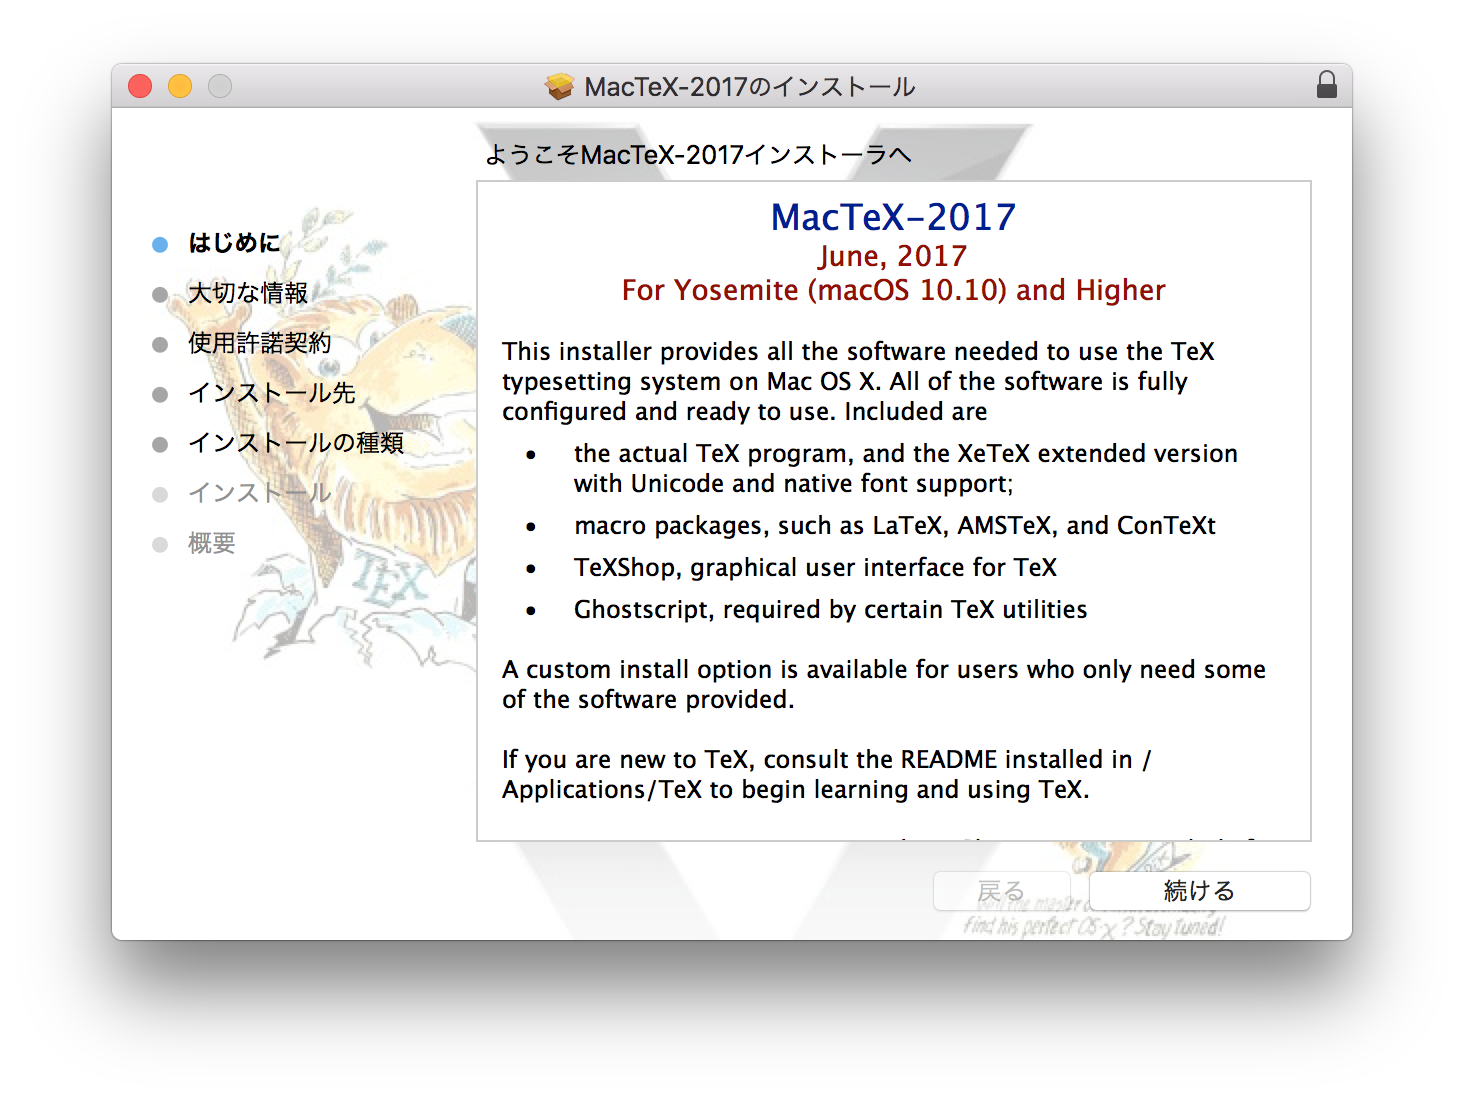
\includegraphics[width=10cm, ]{figs/image.png}
%   \end{center}
% \end{figure}
